

\section{Regression Strategies}


\begin{frame}
    \frametitle{Regression Strategies}

    There are two reasons why we are often not satisfied with the least squares estimates:

    \begin{itemize}

        \item Prediction accuracy: The least squares estimates often have low bias but large variance;

        \item Interpretation: With a large number of predictors (parameters), we often would like to
        determine a smaller subset that exhibit the strogest effects. 
        In order to get the big picture, we are willing to sacrifice some of the small details.

    \end{itemize}

    Strategies to improve the model behavior:

    \begin{itemize}

        \item Player with inputs: Selecting the best combination of inputs to archive the best model;

        \item Adapt the loss function

    \end{itemize}

\end{frame}



\begin{frame}
    \frametitle{Bias and Variance Tradeoff}
    \begin{figure}
        \centering
        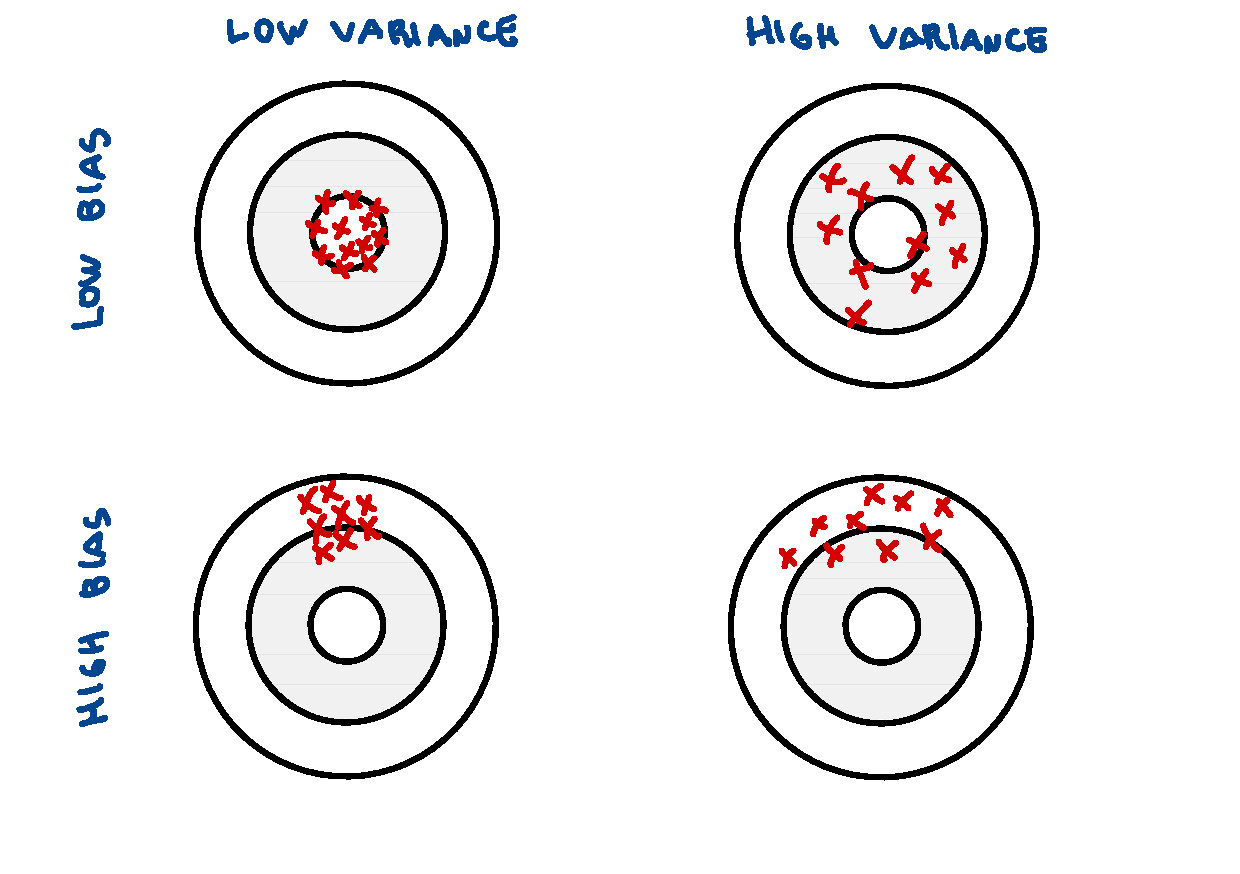
\includegraphics[width=0.95\textwidth]{sections/strategies/figures/bias_variance_tradeoff.pdf}
    \end{figure}
\end{frame}


\subsection {Subset Selection Techniques}


\subsubsection {Best-Subset Selection}
\begin{frame}
    \frametitle{Best-Subset Selection}

    \begin{itemize}

        \item Best subset selection finds for each $k\in{0,1,2,...,p}$ the subset of size $k$
        that gives smallest residual sum of squares;

        \item The question how to choose $k$ involves the tradeoff between bias and variance;

        \item Computation cost: For large $p$ we cannot compute the best subset selection;

        \item Statistical: a price is paid in variance for selecting the best subset of eash size.

    \end{itemize}
\end{frame}


\begin{frame}
    \frametitle{Best-Selection Subset: Example with $k=3$}
    \begin{figure}
        \centering
        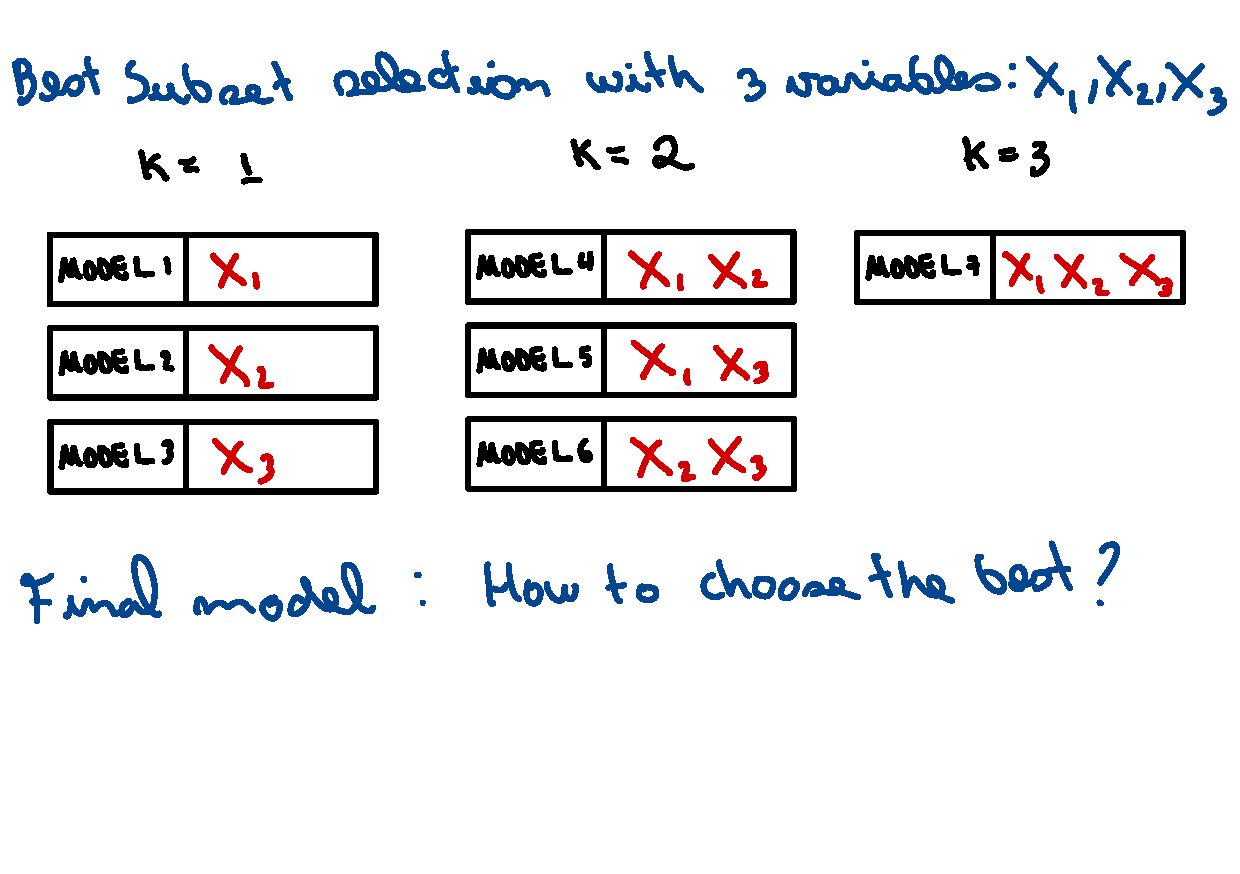
\includegraphics[width=0.95\textwidth]{sections/strategies/figures/best_selection_example.pdf}
    \end{figure}
\end{frame}


\begin{frame}
    \frametitle{Best-Selection Subset: AIC Criterion}
  
    \begin{itemize}
        \item Akaike information Criterion (AIC) is the most popular score to evaluate
        the quality of the model given the least square and the number of parameters $k$:

        $$score = 2k + Nln(LS)$$

        Where with $K$ increase (more complex model), the score increase. However, 
        while an increase (worst fit) in LS has always the same effect

        \item The best model will archive the lowest score. 
    \end{itemize}

\end{frame}




\subsubsection {Forward and Backward-Stepwise Selection}

\begin{frame}
    \frametitle{Forward Stepwise Selection}

    \begin{itemize}

        \item Starts with the intercept ($\beta_0$), and sequentially adds into the model
        the predictor ($\beta_i, X_i$) that most inprove the fit;

        \item For all variables ($X_i$) available:
        \begin{itemize}
            \item Add the most significant variable;
            \item Keep adding the most significant variable until reaching the stopping criterion or
            running out of the variables;
        \end{itemize}

    \end{itemize}
\end{frame}


\begin{frame}
    \frametitle{Forward Stepwise Selection}

    \begin{itemize}

        \item \textbf{The most significant variables:} Let's considere a model tuned with all variables.
        
        \begin{itemize}
            \item For each variable $i$, let's deactivate (force $\beta_i = 0$) and check the impact in the
            model's answer (Least square or AIC score);
            \item The most significant variable will increase (high impact) a lot the LS (Or AIC score);
            \item We can use this strategy to rank each variable;
        \end{itemize}

        \item \textbf{Stopping criterion:} Stop when p-value larger than some specified threshold. The threshold
        can be a fixed value or determined by AIC criterion for each interation.

    \end{itemize}
\end{frame}




\begin{frame}
    \frametitle{Backward Stepwise Selection}

    \begin{itemize}



        \item Use the inverse procedure presented in forward stepwise algorithm;

        \item Starts with the full model, and sequentially deletes the predictor that has the least 
        impact on the fit;
        
        \item Keep dropping the least significant variable until reaching the stopping criterion
        or running out of variables;

        \item Stopping rule is satisfied when all remaining variables inthe model have p-value
        smaller thand some pre-specified threshold all running out; As the forward algorithm, 
        the threshold can be fixed or determined by AIC criterion.

    \end{itemize}
\end{frame}



\subsection {Shrinkage Methods}

\subsubsection{Ridge Regression}

\begin{frame}
    \frametitle{Shrinkage Methods: Ridge Regression}
 
    \begin{itemize}
        \item Ridge regression shrinks the regression coefficients by imposing a 
        penalty (regularization term) on their size;

        \item We always need to find some $\hat{\beta}$ that minimize the least square (LS);

        \item An equivalent way to write the ridge problem is:

        $$L_{ridge}(\hat{\beta}) = \sum_{i=1}^{N}\left(y_i - \beta_0 - \sum_{j=1}^{p}x_{ij}\beta_j\right)^2 {\color{red} + \lambda\sum_{j=1}^{p}\beta_{j}^{2} }$$ 
        
        Here $\lambda\geqslant 0$ is a complexity parameter that controls the amount of shrinkage.

        \item The idea of penalizating by the sum-of-squares of the parameters is also used in 
        neural networks (called as L2 regularization).


    \end{itemize}

\end{frame}


\begin{frame}
    \frametitle{Shrinkage Methods: Ridge Regression}
 
    Once again, let's derive this function:

    \small
    $$L(\beta) = (Y-X\beta)^T(Y-X\beta) {\color{red}+ \lambda\beta^T\beta} = Y^TY - 2\beta^TX^TY + \beta^TX^TX\beta {\color{red}+ \lambda\beta^T\beta}$$

    $$\frac{\delta~L(\beta)}{\delta\beta} = -2X^TY + 2X^TX\beta {\color{red}+2\lambda\beta} = 0$$

    Where the analytical solution must statisfies the normal equation:

    $$ 2X^T(Y - X\beta) = 2\labda\beta \Rightarrow {\color{red}\hat{\beta} = (I\lambda + X^TX)^{-1}X^TY}$$

    Common softwares like $sklearn$ uses the analytical solution to find the $\hat{\beta}$ and 
    some numerical strategies to find the inverse matrix.

\end{frame}



\subsubsection {Lasso Regression}


\begin{frame}
    \frametitle{Shrinkage Methods: Lasso Regression}
 
    \begin{itemize}
        \item Lasso regression shrinks the regression coefficients by imposing a 
        L1 penalty (regularization term) on their size;

        \item We always need to find some $\hat{\beta}$ that minimize the least square (LS);

        \item An equivalent way to write the ridge problem is:

        $$L_{lasso}(\hat{\beta}) = \sum_{i=1}^{N}\left(y_i - \beta_0 - \sum_{j=1}^{p}x_{ij}\beta_j\right)^2 {\color{red} + \lambda\sum_{j=1}^{p}|\beta_{j}| }$$ 

        Where the L2 ridge penalty is replaced by the L1 lasso penalty.

    \end{itemize}

\end{frame}
